% Options for packages loaded elsewhere
\PassOptionsToPackage{unicode}{hyperref}
\PassOptionsToPackage{hyphens}{url}
%
\documentclass[
]{article}
\usepackage{lmodern}
\usepackage{amsmath}
\usepackage{ifxetex,ifluatex}
\ifnum 0\ifxetex 1\fi\ifluatex 1\fi=0 % if pdftex
  \usepackage[T1]{fontenc}
  \usepackage[utf8]{inputenc}
  \usepackage{textcomp} % provide euro and other symbols
  \usepackage{amssymb}
\else % if luatex or xetex
  \usepackage{unicode-math}
  \defaultfontfeatures{Scale=MatchLowercase}
  \defaultfontfeatures[\rmfamily]{Ligatures=TeX,Scale=1}
\fi
% Use upquote if available, for straight quotes in verbatim environments
\IfFileExists{upquote.sty}{\usepackage{upquote}}{}
\IfFileExists{microtype.sty}{% use microtype if available
  \usepackage[]{microtype}
  \UseMicrotypeSet[protrusion]{basicmath} % disable protrusion for tt fonts
}{}
\makeatletter
\@ifundefined{KOMAClassName}{% if non-KOMA class
  \IfFileExists{parskip.sty}{%
    \usepackage{parskip}
  }{% else
    \setlength{\parindent}{0pt}
    \setlength{\parskip}{6pt plus 2pt minus 1pt}}
}{% if KOMA class
  \KOMAoptions{parskip=half}}
\makeatother
\usepackage{xcolor}
\IfFileExists{xurl.sty}{\usepackage{xurl}}{} % add URL line breaks if available
\IfFileExists{bookmark.sty}{\usepackage{bookmark}}{\usepackage{hyperref}}
\hypersetup{
  pdftitle={Data Visualization Final Paper},
  pdfauthor={Shreyas Meher},
  hidelinks,
  pdfcreator={LaTeX via pandoc}}
\urlstyle{same} % disable monospaced font for URLs
\usepackage[margin=1in]{geometry}
\usepackage{color}
\usepackage{fancyvrb}
\newcommand{\VerbBar}{|}
\newcommand{\VERB}{\Verb[commandchars=\\\{\}]}
\DefineVerbatimEnvironment{Highlighting}{Verbatim}{commandchars=\\\{\}}
% Add ',fontsize=\small' for more characters per line
\usepackage{framed}
\definecolor{shadecolor}{RGB}{248,248,248}
\newenvironment{Shaded}{\begin{snugshade}}{\end{snugshade}}
\newcommand{\AlertTok}[1]{\textcolor[rgb]{0.94,0.16,0.16}{#1}}
\newcommand{\AnnotationTok}[1]{\textcolor[rgb]{0.56,0.35,0.01}{\textbf{\textit{#1}}}}
\newcommand{\AttributeTok}[1]{\textcolor[rgb]{0.77,0.63,0.00}{#1}}
\newcommand{\BaseNTok}[1]{\textcolor[rgb]{0.00,0.00,0.81}{#1}}
\newcommand{\BuiltInTok}[1]{#1}
\newcommand{\CharTok}[1]{\textcolor[rgb]{0.31,0.60,0.02}{#1}}
\newcommand{\CommentTok}[1]{\textcolor[rgb]{0.56,0.35,0.01}{\textit{#1}}}
\newcommand{\CommentVarTok}[1]{\textcolor[rgb]{0.56,0.35,0.01}{\textbf{\textit{#1}}}}
\newcommand{\ConstantTok}[1]{\textcolor[rgb]{0.00,0.00,0.00}{#1}}
\newcommand{\ControlFlowTok}[1]{\textcolor[rgb]{0.13,0.29,0.53}{\textbf{#1}}}
\newcommand{\DataTypeTok}[1]{\textcolor[rgb]{0.13,0.29,0.53}{#1}}
\newcommand{\DecValTok}[1]{\textcolor[rgb]{0.00,0.00,0.81}{#1}}
\newcommand{\DocumentationTok}[1]{\textcolor[rgb]{0.56,0.35,0.01}{\textbf{\textit{#1}}}}
\newcommand{\ErrorTok}[1]{\textcolor[rgb]{0.64,0.00,0.00}{\textbf{#1}}}
\newcommand{\ExtensionTok}[1]{#1}
\newcommand{\FloatTok}[1]{\textcolor[rgb]{0.00,0.00,0.81}{#1}}
\newcommand{\FunctionTok}[1]{\textcolor[rgb]{0.00,0.00,0.00}{#1}}
\newcommand{\ImportTok}[1]{#1}
\newcommand{\InformationTok}[1]{\textcolor[rgb]{0.56,0.35,0.01}{\textbf{\textit{#1}}}}
\newcommand{\KeywordTok}[1]{\textcolor[rgb]{0.13,0.29,0.53}{\textbf{#1}}}
\newcommand{\NormalTok}[1]{#1}
\newcommand{\OperatorTok}[1]{\textcolor[rgb]{0.81,0.36,0.00}{\textbf{#1}}}
\newcommand{\OtherTok}[1]{\textcolor[rgb]{0.56,0.35,0.01}{#1}}
\newcommand{\PreprocessorTok}[1]{\textcolor[rgb]{0.56,0.35,0.01}{\textit{#1}}}
\newcommand{\RegionMarkerTok}[1]{#1}
\newcommand{\SpecialCharTok}[1]{\textcolor[rgb]{0.00,0.00,0.00}{#1}}
\newcommand{\SpecialStringTok}[1]{\textcolor[rgb]{0.31,0.60,0.02}{#1}}
\newcommand{\StringTok}[1]{\textcolor[rgb]{0.31,0.60,0.02}{#1}}
\newcommand{\VariableTok}[1]{\textcolor[rgb]{0.00,0.00,0.00}{#1}}
\newcommand{\VerbatimStringTok}[1]{\textcolor[rgb]{0.31,0.60,0.02}{#1}}
\newcommand{\WarningTok}[1]{\textcolor[rgb]{0.56,0.35,0.01}{\textbf{\textit{#1}}}}
\usepackage{graphicx}
\makeatletter
\def\maxwidth{\ifdim\Gin@nat@width>\linewidth\linewidth\else\Gin@nat@width\fi}
\def\maxheight{\ifdim\Gin@nat@height>\textheight\textheight\else\Gin@nat@height\fi}
\makeatother
% Scale images if necessary, so that they will not overflow the page
% margins by default, and it is still possible to overwrite the defaults
% using explicit options in \includegraphics[width, height, ...]{}
\setkeys{Gin}{width=\maxwidth,height=\maxheight,keepaspectratio}
% Set default figure placement to htbp
\makeatletter
\def\fps@figure{htbp}
\makeatother
\setlength{\emergencystretch}{3em} % prevent overfull lines
\providecommand{\tightlist}{%
  \setlength{\itemsep}{0pt}\setlength{\parskip}{0pt}}
\setcounter{secnumdepth}{-\maxdimen} % remove section numbering
\ifluatex
  \usepackage{selnolig}  % disable illegal ligatures
\fi
\newlength{\cslhangindent}
\setlength{\cslhangindent}{1.5em}
\newlength{\csllabelwidth}
\setlength{\csllabelwidth}{3em}
\newenvironment{CSLReferences}[2] % #1 hanging-ident, #2 entry spacing
 {% don't indent paragraphs
  \setlength{\parindent}{0pt}
  % turn on hanging indent if param 1 is 1
  \ifodd #1 \everypar{\setlength{\hangindent}{\cslhangindent}}\ignorespaces\fi
  % set entry spacing
  \ifnum #2 > 0
  \setlength{\parskip}{#2\baselineskip}
  \fi
 }%
 {}
\usepackage{calc}
\newcommand{\CSLBlock}[1]{#1\hfill\break}
\newcommand{\CSLLeftMargin}[1]{\parbox[t]{\csllabelwidth}{#1}}
\newcommand{\CSLRightInline}[1]{\parbox[t]{\linewidth - \csllabelwidth}{#1}\break}
\newcommand{\CSLIndent}[1]{\hspace{\cslhangindent}#1}

\title{Data Visualization Final Paper}
\author{Shreyas Meher}
\date{12/4/2021}

\begin{document}
\maketitle

\begin{Shaded}
\begin{Highlighting}[]
\NormalTok{knitr}\SpecialCharTok{::}\NormalTok{opts\_chunk}\SpecialCharTok{$}\FunctionTok{set}\NormalTok{(}\AttributeTok{warning =} \ConstantTok{FALSE}\NormalTok{, }\AttributeTok{message =} \ConstantTok{FALSE}\NormalTok{) }

\FunctionTok{library}\NormalTok{(flexdashboard)}
\NormalTok{footprint }\OtherTok{\textless{}{-}} \FunctionTok{read.csv}\NormalTok{(}\StringTok{"countries.csv"}\NormalTok{)}

\FunctionTok{library}\NormalTok{(dplyr) }\CommentTok{\# data wrangling}
\FunctionTok{library}\NormalTok{(tidyr) }\CommentTok{\# data wrangling}
\FunctionTok{library}\NormalTok{(ggplot2) }\CommentTok{\# plot}
\FunctionTok{library}\NormalTok{(plotly) }\CommentTok{\# interactive plot}
\FunctionTok{library}\NormalTok{(ggthemes) }\CommentTok{\# themes for ggplot2}
\FunctionTok{library}\NormalTok{(extrafont) }\CommentTok{\# fonts for ggplot2}
\FunctionTok{library}\NormalTok{(RColorBrewer) }\CommentTok{\# colors}
\end{Highlighting}
\end{Shaded}

\hypertarget{introduction}{%
\subsection{Introduction}\label{introduction}}

There has been considerable research done on the ecological impact of
the growing consumption patterns all across the world (Toth and Szigeti
2016). The theory follows Malthusian concepts and tenets, wherein the
developed world and now the developing nations are increasing their
consumption of resources available in the environment for a marginal
increase in economic growth and development. Malthus decried the
explosive population growth and the strain that it caused on the
resources, thus leading to a stagnation in world income and income per
capita. Operationalization of the ability of certain countries to
recover resources and their rate of exhaustion of resources is another
question, and is the focus of the Global Footprint Network (GFN), which
is the data-set used for this project.

This project is exploratory in nature, and looks to see how Bio-capacity
and Ecological Footprint and the relationship between them and various
other variables plays out using the GFN database. The main purpose for
this paper lies in the question regarding sustainable development goals
and whether consumption patterns around the world are indeed changing.
For this, various data visualization methods as gleaned from the class
will be used for the purposes of this paper.

\hypertarget{variable-definitions}{%
\subsection{Variable definitions}\label{variable-definitions}}

To get us started off, I will mention key definitions that are crucial
to understand for this project. The GFN have defined the variables,
which is what I am noting down in this section.

\textbf{Ecological Footprint} - A measure of how much area of
biologically productive land and water an individual, population, or
activity requires to produce all the resources it consumes and to absorb
the waste it generates, using prevailing technology and resource
management practices. The Ecological Footprint is usually measured in
global hectares. Because trade is global, an individual or country's
Footprint includes land or sea from all over the world. Without further
specification, Ecological Footprint generally refers to the Ecological
Footprint of consumption. Ecological Footprint is often referred to in
short form as Footprint.

\textbf{Biocapacity} - The capacity of ecosystems to regenerate what
people demand from those surfaces. Life, including human life, competes
for space. The biocapacity of a surface represents its ability to renew
what people demand. Biocapacity is therefore the ecosystems' capacity to
produce biological materials used by people and to absorb waste material
generated by humans, under current management schemes and extraction
technologies. Biocapacity can change from year to year due to climate,
management, and proportion considered useful inputs to the human
economy. In the National Footprint and Biocapacity Accounts, biocapacity
is calculated by multiplying the physical area by the yield factor and
the appropriate equivalence factor. Biocapacity is expressed in global
hectares.

\textbf{Global Hectares (gha)} - Global hectares are the accounting unit
for the Ecological Footprint and biocapacity accounts. These
productivity weighted biologically productive hectares allow researchers
to report both the biocapacity of the earth or a region and the demand
on biocapacity (the Ecological Footprint). A global hectare is a
biologically productive hectare with world average biological
productivity for a given year. Global hectares are useful because
different land types have different productivities. A global hectare of
cropland, for example, would occupy a smaller physical area than the
much less biologically productive pasture land, as more pasture would be
needed to provide the same biocapacity as one hectare of cropland.
Because world productivity varies slightly from year to year, the value
of a global hectare may change slightly from year to year.

\textbf{Ecological Deficit/Reserve} - The difference between the
biocapacity and Ecological Footprint of a region or country. An
ecological deficit occurs when the Footprint of a population exceeds the
biocapacity of the area available to that population. Conversely, an
ecological reserve exists when the biocapacity of a region exceeds its
population's Footprint. If there is a regional or national ecological
deficit, it means that the region is importing biocapacity through trade
or liquidating regional ecological assets, or emitting wastes into the
global commons such as the atmosphere. In contrast to the national
scale, the global ecological deficit cannot be compensated for through
trade, and is therefore equal to overshoot by definition.

\hypertarget{data-exploration-boxplots}{%
\subsection{Data Exploration
(Boxplots)}\label{data-exploration-boxplots}}

First, the data has to be explored so that we have a good representation
of the Biocapacity and Ecological Footprint of the nations. Doing this
for all the countries in the dataset will be difficult to visualize
clearly, and so the region of the country will be used as a factor to
help. Visualizing the regions with the help of boxplots is useful as it
gives us a good indication of the variance within and between regions at
the same time.

The two plots here show the Ecological Footprint and Biocapacity for all
regions in the study. Here we can see that there exists a lot of
variance between and within regions, with certain regions having high
Ecological Footprints and low Biocapacity and vice versa. This however
does not help with understanding the certain countries which might be
outliers in both variables of concern. And so, we will have to filter
the dataset to see the top 10 countries for both variables - which is
the next section of this exploratory analysis. We can clearly see the
difference in Ecological Footprint versus the Biocapacity of the various
regions in the world. Here, we can tell that the European Union, on
account of the number of developed nations it consists of along with
Central Asia have the largest Ecological Footprint.

\hypertarget{total-ecological-footprint-by-region}{%
\subsubsection{Total Ecological Footprint by
region}\label{total-ecological-footprint-by-region}}

\begin{Shaded}
\begin{Highlighting}[]
\NormalTok{p2}\OtherTok{\textless{}{-}} \FunctionTok{ggplot}\NormalTok{(footprint) }\SpecialCharTok{+}
  \FunctionTok{aes}\NormalTok{(}\AttributeTok{x =} \StringTok{""}\NormalTok{, }\AttributeTok{y =}\NormalTok{ Total.Ecological.Footprint, }\AttributeTok{colour =}\NormalTok{ Region) }\SpecialCharTok{+}
  \FunctionTok{geom\_boxplot}\NormalTok{(}\AttributeTok{shape =} \StringTok{"circle"}\NormalTok{, }\AttributeTok{fill =} \StringTok{"\#ffffff"}\NormalTok{) }\SpecialCharTok{+}
  \FunctionTok{scale\_color\_brewer}\NormalTok{(}\AttributeTok{palette =} \StringTok{"Set2"}\NormalTok{, }\AttributeTok{direction =} \DecValTok{1}\NormalTok{) }\SpecialCharTok{+}
  \FunctionTok{labs}\NormalTok{(}
    \AttributeTok{x =} \StringTok{"Region"}\NormalTok{,}
    \AttributeTok{y =} \StringTok{"Ecological Footprint (Global Hectares)"}\NormalTok{,}
    \AttributeTok{title =} \StringTok{"Total Ecological Footprint by region"}
\NormalTok{  ) }\SpecialCharTok{+}
\NormalTok{  ggthemes}\SpecialCharTok{::}\FunctionTok{theme\_gdocs}\NormalTok{() }\SpecialCharTok{+}
  \FunctionTok{theme}\NormalTok{(}\AttributeTok{plot.title =} \FunctionTok{element\_text}\NormalTok{(}\AttributeTok{hjust =} \FloatTok{0.5}\NormalTok{)) }\SpecialCharTok{+} \FunctionTok{theme}\NormalTok{(}\AttributeTok{axis.title =} \FunctionTok{element\_text}\NormalTok{(}\AttributeTok{family =} \StringTok{"serif"}\NormalTok{),}
    \AttributeTok{axis.text =} \FunctionTok{element\_text}\NormalTok{(}\AttributeTok{family =} \StringTok{"serif"}\NormalTok{),}
    \AttributeTok{axis.text.x =} \FunctionTok{element\_text}\NormalTok{(}\AttributeTok{family =} \StringTok{"serif"}\NormalTok{),}
    \AttributeTok{axis.text.y =} \FunctionTok{element\_text}\NormalTok{(}\AttributeTok{family =} \StringTok{"serif"}\NormalTok{),}
    \AttributeTok{plot.title =} \FunctionTok{element\_text}\NormalTok{(}\AttributeTok{family =} \StringTok{"serif"}\NormalTok{,}
        \AttributeTok{size =} \DecValTok{15}\NormalTok{, }\AttributeTok{colour =} \StringTok{"black"}\NormalTok{), }\AttributeTok{legend.text =} \FunctionTok{element\_text}\NormalTok{(}\AttributeTok{family =} \StringTok{"serif"}\NormalTok{),}
    \AttributeTok{legend.title =} \FunctionTok{element\_text}\NormalTok{(}\AttributeTok{family =} \StringTok{"serif"}\NormalTok{)) }\SpecialCharTok{+} \FunctionTok{theme}\NormalTok{(}\AttributeTok{axis.title =} \FunctionTok{element\_text}\NormalTok{(}\AttributeTok{colour =} \StringTok{"black"}\NormalTok{))}

\NormalTok{p2 }
\end{Highlighting}
\end{Shaded}

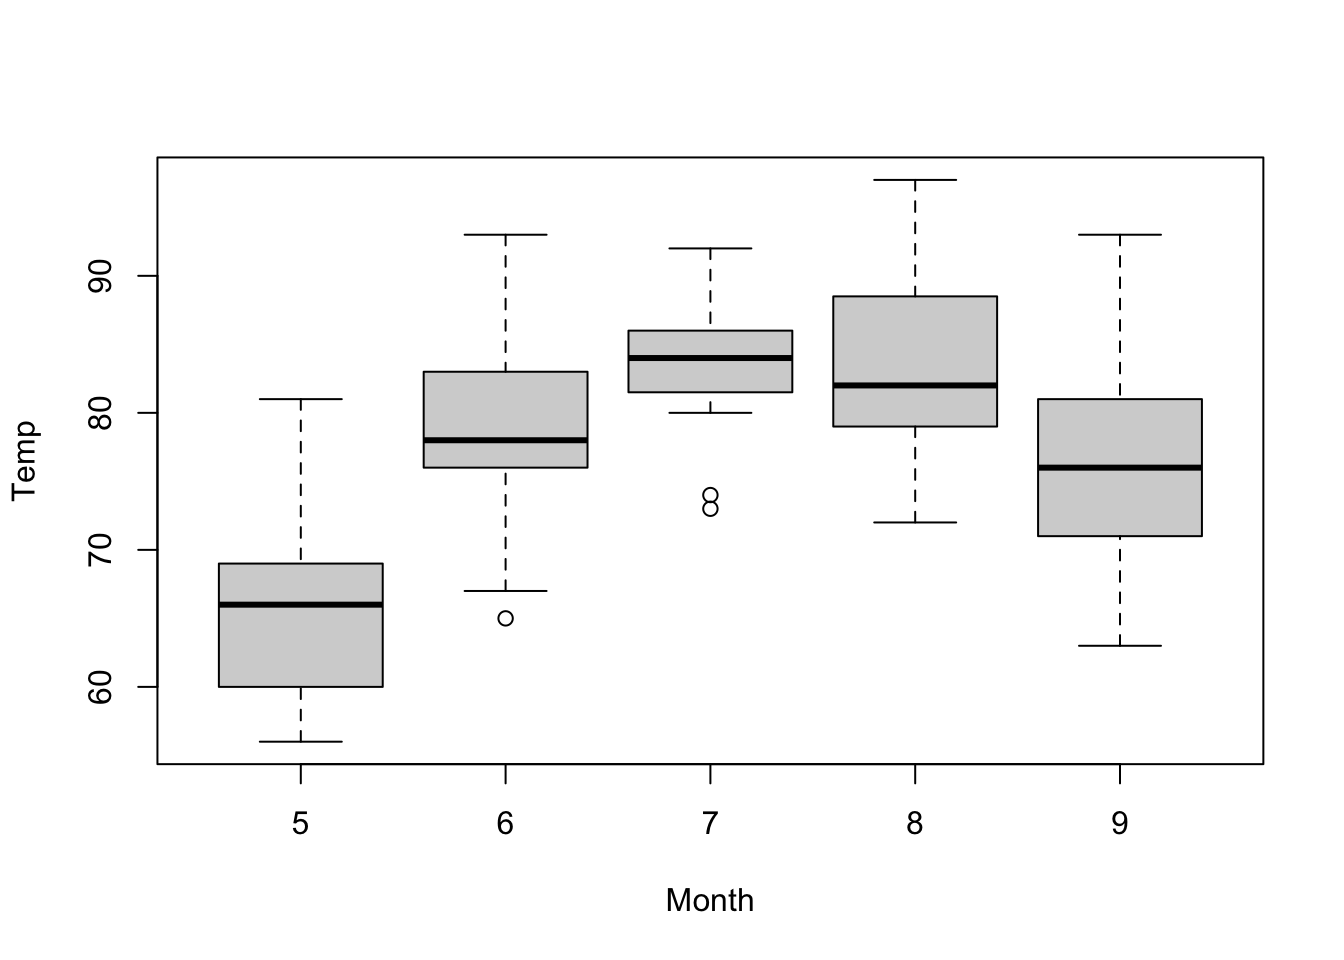
\includegraphics{footprint-paper_files/figure-latex/unnamed-chunk-1-1.pdf}

\hypertarget{total-biocapacity-by-region}{%
\subsubsection{Total Biocapacity by
Region}\label{total-biocapacity-by-region}}

\begin{Shaded}
\begin{Highlighting}[]
\NormalTok{p3}\OtherTok{\textless{}{-}} \FunctionTok{ggplot}\NormalTok{(footprint) }\SpecialCharTok{+}
  \FunctionTok{aes}\NormalTok{(}\AttributeTok{x =} \StringTok{""}\NormalTok{, }\AttributeTok{y =}\NormalTok{ Total.Biocapacity, }\AttributeTok{colour =}\NormalTok{ Region) }\SpecialCharTok{+}
  \FunctionTok{geom\_boxplot}\NormalTok{(}\AttributeTok{shape =} \StringTok{"circle"}\NormalTok{, }\AttributeTok{fill =} \StringTok{"\#ffffff"}\NormalTok{) }\SpecialCharTok{+}
  \FunctionTok{scale\_color\_brewer}\NormalTok{(}\AttributeTok{palette =} \StringTok{"Set2"}\NormalTok{, }\AttributeTok{direction =} \DecValTok{1}\NormalTok{) }\SpecialCharTok{+}
  \FunctionTok{labs}\NormalTok{(}
    \AttributeTok{x =} \StringTok{"Region"}\NormalTok{,}
    \AttributeTok{y =} \StringTok{"Biocapacity (Global Hectares)"}\NormalTok{,}
    \AttributeTok{title =} \StringTok{"Total Biocapacity by region"}
\NormalTok{  ) }\SpecialCharTok{+}
\NormalTok{  ggthemes}\SpecialCharTok{::}\FunctionTok{theme\_gdocs}\NormalTok{() }\SpecialCharTok{+} \FunctionTok{theme}\NormalTok{(}\AttributeTok{axis.title =} \FunctionTok{element\_text}\NormalTok{(}\AttributeTok{family =} \StringTok{"serif"}\NormalTok{,}
    \AttributeTok{colour =} \StringTok{"black"}\NormalTok{), }\AttributeTok{axis.text =} \FunctionTok{element\_text}\NormalTok{(}\AttributeTok{family =} \StringTok{"serif"}\NormalTok{),}
    \AttributeTok{axis.text.x =} \FunctionTok{element\_text}\NormalTok{(}\AttributeTok{family =} \StringTok{"serif"}\NormalTok{),}
    \AttributeTok{axis.text.y =} \FunctionTok{element\_text}\NormalTok{(}\AttributeTok{family =} \StringTok{"serif"}\NormalTok{),}
    \AttributeTok{plot.title =} \FunctionTok{element\_text}\NormalTok{(}\AttributeTok{family =} \StringTok{"serif"}\NormalTok{,}
        \AttributeTok{size =} \DecValTok{15}\NormalTok{, }\AttributeTok{colour =} \StringTok{"black"}\NormalTok{, }\AttributeTok{hjust =} \FloatTok{0.5}\NormalTok{),}
    \AttributeTok{legend.text =} \FunctionTok{element\_text}\NormalTok{(}\AttributeTok{family =} \StringTok{"serif"}\NormalTok{),}
    \AttributeTok{legend.title =} \FunctionTok{element\_text}\NormalTok{(}\AttributeTok{family =} \StringTok{"serif"}\NormalTok{))}

\NormalTok{p3 }\SpecialCharTok{+} \FunctionTok{ylim}\NormalTok{(}\DecValTok{0}\NormalTok{,}\DecValTok{17}\NormalTok{)}
\end{Highlighting}
\end{Shaded}

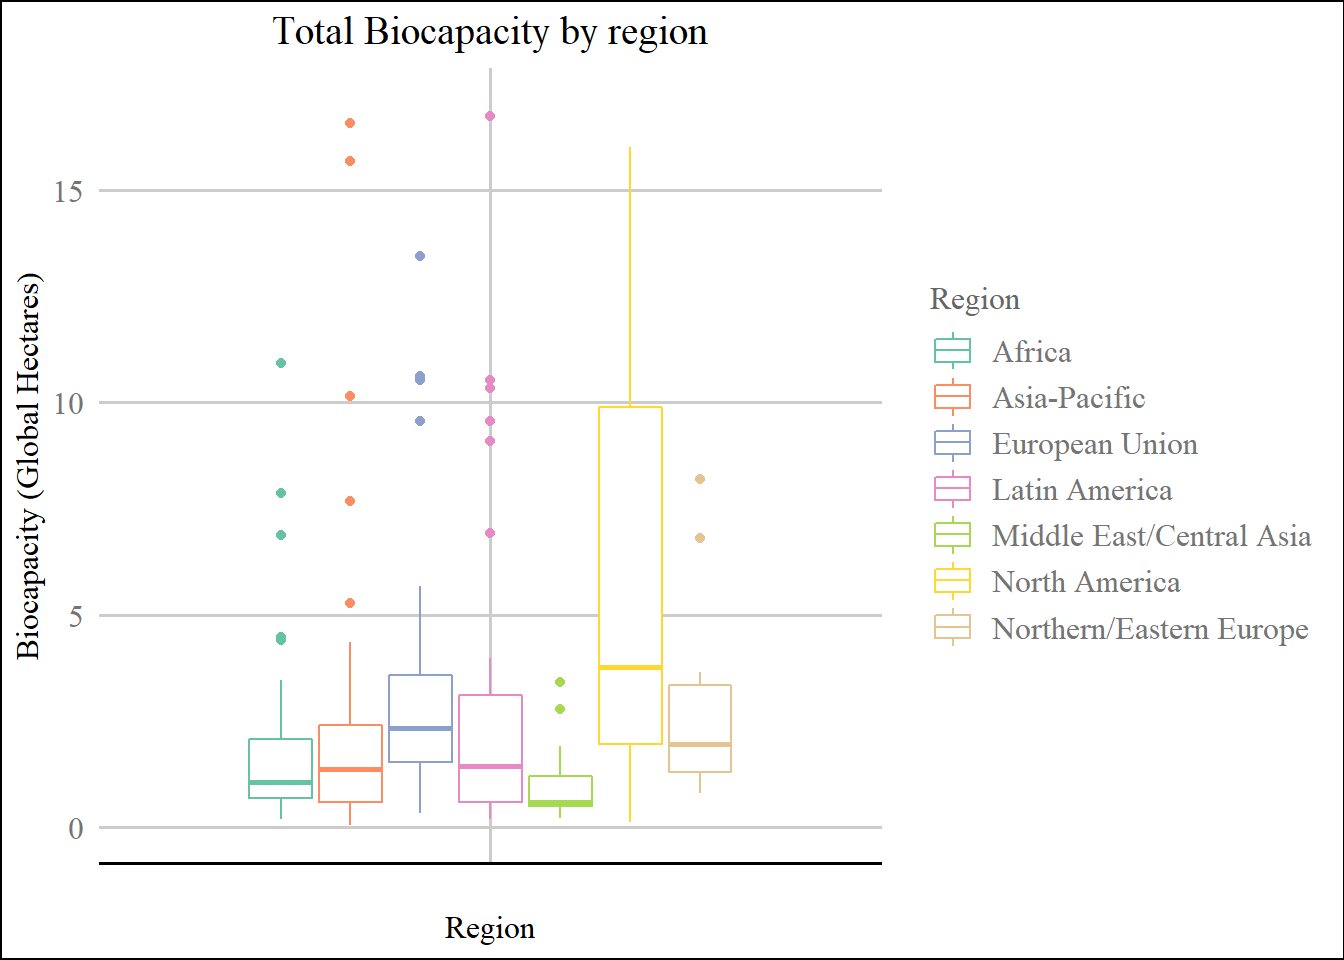
\includegraphics{footprint-paper_files/figure-latex/unnamed-chunk-2-1.pdf}

\hypertarget{data-exploration-top-10-analysis}{%
\subsection{Data Exploration (Top 10
Analysis)}\label{data-exploration-top-10-analysis}}

Here, we create a list with the top 10 countries for each variable
(Ecological Footprint \& Biocapacity) using the top\_n function from the
\emph{dplyr} library. Using these lists, we can then plot simple bar
charts to give us a deeper look into the countries at the outliers of
our data, which have either extremely high Ecological Footprints or high
Biocapacities.

From the resultant plot, we can see that most of the countries in the
top 10 of Ecological Footprint data are developed nations - with only
Qatar, Trinidad and Tobago and Oman being the lesser developed of the
10. This is corroborated by research by Galli et al. (2012) and other
researchers who find out that the developed world has a few factors
which lead to overuse of natural resources due to industrialization and
a better ability at extracting resources more efficiently. Luxembourg
and Qatar stand out as having higher Ecological Footprints than all the
rest of the outliers. Luxembourg is one of the smallest nations in and
has one of the smallest population sizes in Europe. Yet, the country's
carbon footprint on a per capita basis is significantly higher than that
of any other European nation. A big contributor to Luxembourg's
catastrophic carbon emissions is the car ownership rate as well as
energy consumption per capita, which are both the highest in Europe.
Luxembourg does not have a lot of energy being consumed from renewable
sources (2.1\%), which adds to the negative carbon balance. This
analysis is however controversial in academic circles, where certain
researchers believe that there exists a discrepancy between the data
reported by the GFN and the actual data in Luxembourg and other
countries Hild et al. (2010).

\hypertarget{top-10-ecological-footprint-countries}{%
\subsubsection{Top 10 Ecological Footprint
countries}\label{top-10-ecological-footprint-countries}}

\begin{Shaded}
\begin{Highlighting}[]
\NormalTok{top\_10 }\OtherTok{\textless{}{-}} \FunctionTok{top\_n}\NormalTok{(footprint, }\AttributeTok{n=}\DecValTok{10}\NormalTok{, Total.Ecological.Footprint) }\SpecialCharTok{\%\textgreater{}\%} 
  \FunctionTok{arrange}\NormalTok{(}\FunctionTok{desc}\NormalTok{(Total.Ecological.Footprint))}


\FunctionTok{ggplot}\NormalTok{(top\_10,}\FunctionTok{aes}\NormalTok{(}\AttributeTok{x=} \FunctionTok{reorder}\NormalTok{(Country, }\SpecialCharTok{{-}}\NormalTok{Total.Ecological.Footprint), }\AttributeTok{y=}\NormalTok{Total.Ecological.Footprint, }\AttributeTok{fill =}\NormalTok{ Total.Ecological.Footprint))}\SpecialCharTok{+}
  \FunctionTok{scale\_fill\_gradient}\NormalTok{(}
    \AttributeTok{low =} \StringTok{"\#fd9aa6"}\NormalTok{,}
    \AttributeTok{high =} \StringTok{"\#FB0421"}\NormalTok{,}
    \AttributeTok{space =} \StringTok{"Lab"}\NormalTok{,}
    \AttributeTok{na.value =} \StringTok{"grey50"}\NormalTok{,}
    \AttributeTok{guide =} \StringTok{"colourbar"}\NormalTok{,}
    \AttributeTok{aesthetics =} \StringTok{"fill"}\NormalTok{)}\SpecialCharTok{+} 
  \FunctionTok{geom\_col}\NormalTok{()}\SpecialCharTok{+}
  \FunctionTok{theme}\NormalTok{(}\AttributeTok{axis.text.x =} \FunctionTok{element\_text}\NormalTok{(}\AttributeTok{angle =} \DecValTok{40}\NormalTok{, }\AttributeTok{vjust =} \DecValTok{1}\NormalTok{, }\AttributeTok{hjust =}\DecValTok{1}\NormalTok{),}
        \AttributeTok{legend.position =} \StringTok{"none"}\NormalTok{)}\SpecialCharTok{+}
  
  \CommentTok{\# Changing labels}
  
  \FunctionTok{labs}\NormalTok{(}\AttributeTok{y =} \StringTok{"Total Ecological Footprint (Global Hectares)"}\NormalTok{,}
       \AttributeTok{x =} \StringTok{\textquotesingle{}\textquotesingle{}}\NormalTok{,}
       \AttributeTok{title =} \StringTok{"Highest Ecological Footprint Countries"}\NormalTok{,}
       \AttributeTok{caption =} \StringTok{\textquotesingle{}Source: Global Ecoogical Footprint, Global Footprint Network\textquotesingle{}}\NormalTok{)}\SpecialCharTok{+}
    \FunctionTok{theme}\NormalTok{(}\AttributeTok{plot.subtitle =} \FunctionTok{element\_text}\NormalTok{(}\AttributeTok{family =} \StringTok{"serif"}\NormalTok{),}
    \AttributeTok{plot.caption =} \FunctionTok{element\_text}\NormalTok{(}\AttributeTok{family =} \StringTok{"serif"}\NormalTok{),}
    \AttributeTok{panel.grid.major =} \FunctionTok{element\_line}\NormalTok{(}\AttributeTok{colour =} \StringTok{"gray94"}\NormalTok{),}
    \AttributeTok{panel.grid.minor =} \FunctionTok{element\_line}\NormalTok{(}\AttributeTok{colour =} \StringTok{"white"}\NormalTok{),}
    \AttributeTok{axis.title =} \FunctionTok{element\_text}\NormalTok{(}\AttributeTok{family =} \StringTok{"serif"}\NormalTok{),}
    \AttributeTok{plot.title =} \FunctionTok{element\_text}\NormalTok{(}\AttributeTok{family =} \StringTok{"serif"}\NormalTok{,}
        \AttributeTok{size =} \DecValTok{15}\NormalTok{, }\AttributeTok{hjust =} \FloatTok{0.5}\NormalTok{), }\AttributeTok{legend.title =} \FunctionTok{element\_text}\NormalTok{(}\AttributeTok{family =} \StringTok{"serif"}\NormalTok{),}
    \AttributeTok{panel.background =} \FunctionTok{element\_rect}\NormalTok{(}\AttributeTok{fill =} \StringTok{"white"}\NormalTok{,}
        \AttributeTok{colour =} \StringTok{"white"}\NormalTok{)) }\SpecialCharTok{+}\FunctionTok{labs}\NormalTok{(}\AttributeTok{x =} \ConstantTok{NULL}\NormalTok{) }\SpecialCharTok{+} \FunctionTok{theme}\NormalTok{(}\AttributeTok{axis.text =} \FunctionTok{element\_text}\NormalTok{(}\AttributeTok{family =} \StringTok{"serif"}\NormalTok{),}
    \AttributeTok{axis.text.x =} \FunctionTok{element\_text}\NormalTok{(}\AttributeTok{family =} \StringTok{"serif"}\NormalTok{),}
    \AttributeTok{axis.text.y =} \FunctionTok{element\_text}\NormalTok{(}\AttributeTok{family =} \StringTok{"serif"}\NormalTok{),}
    \AttributeTok{legend.text =} \FunctionTok{element\_text}\NormalTok{(}\AttributeTok{family =} \StringTok{"serif"}\NormalTok{))}
\end{Highlighting}
\end{Shaded}

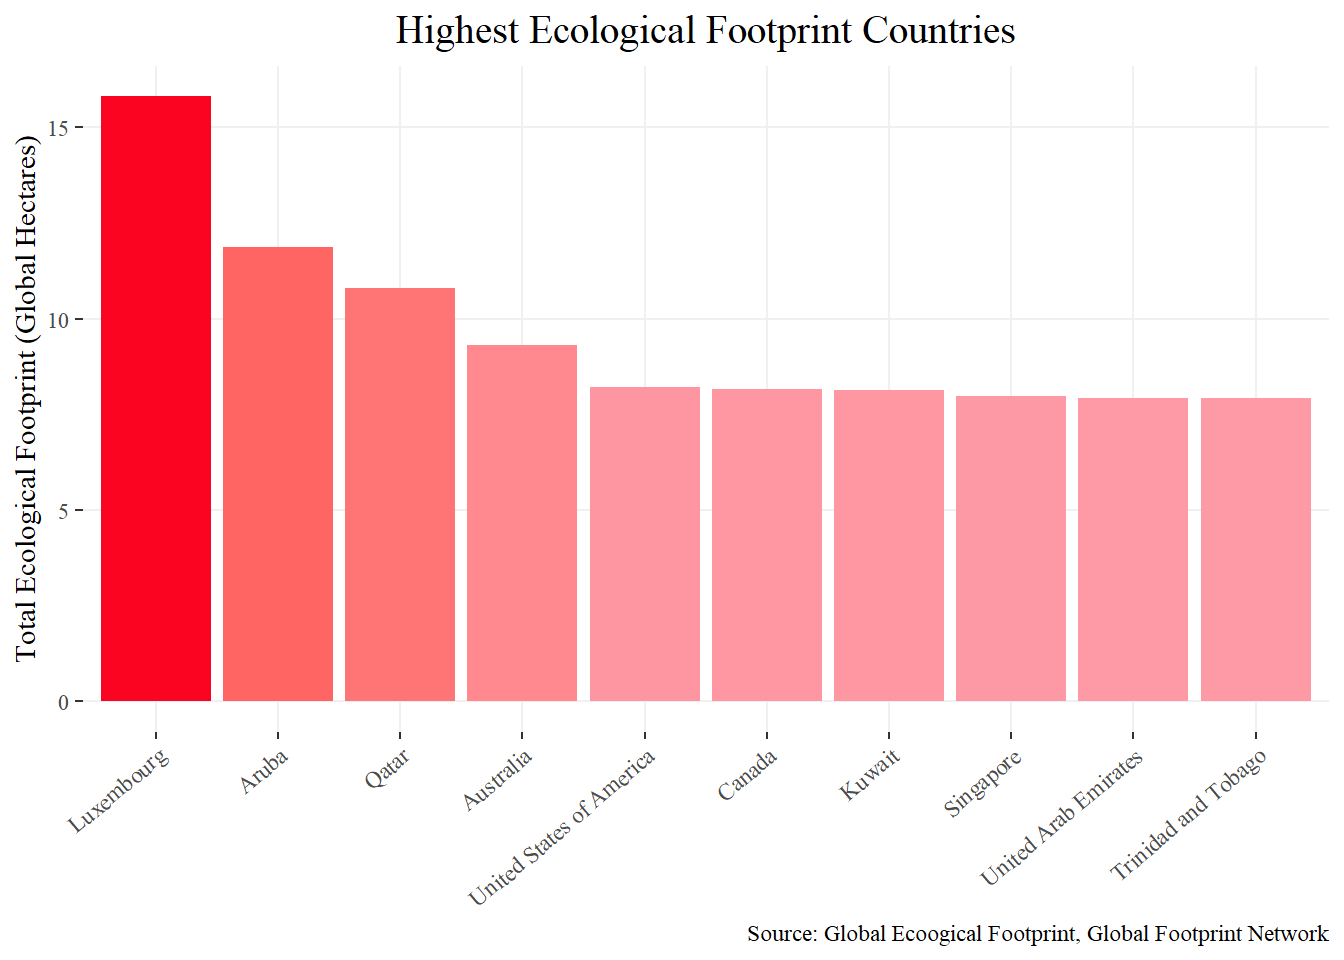
\includegraphics{footprint-paper_files/figure-latex/unnamed-chunk-3-1.pdf}

\hypertarget{top-10-biocapacity-countries}{%
\subsubsection{Top 10 Biocapacity
countries}\label{top-10-biocapacity-countries}}

\begin{Shaded}
\begin{Highlighting}[]
\CommentTok{\# Selecting top 10 countries and arranging by Biocapacity}

\NormalTok{top2\_10 }\OtherTok{\textless{}{-}} \FunctionTok{top\_n}\NormalTok{(footprint, }\AttributeTok{n=}\DecValTok{10}\NormalTok{, Total.Biocapacity) }\SpecialCharTok{\%\textgreater{}\%} 
  \FunctionTok{arrange}\NormalTok{(}\FunctionTok{desc}\NormalTok{(Total.Biocapacity))}

\FunctionTok{ggplot}\NormalTok{(top2\_10,}\FunctionTok{aes}\NormalTok{(}\AttributeTok{x=} \FunctionTok{reorder}\NormalTok{(Country, }\SpecialCharTok{{-}}\NormalTok{Total.Biocapacity), }\AttributeTok{y=}\NormalTok{Total.Biocapacity, }\AttributeTok{fill =}\NormalTok{ Total.Biocapacity))}\SpecialCharTok{+}
  \FunctionTok{scale\_fill\_gradient}\NormalTok{(}
    \AttributeTok{low =} \StringTok{"\#9BC8AE"}\NormalTok{,}
    \AttributeTok{high =} \StringTok{"\#067736"}\NormalTok{,}
    \AttributeTok{space =} \StringTok{"Lab"}\NormalTok{,}
    \AttributeTok{na.value =} \StringTok{"grey50"}\NormalTok{,}
    \AttributeTok{guide =} \StringTok{"colourbar"}\NormalTok{,}
    \AttributeTok{aesthetics =} \StringTok{"fill"}\NormalTok{)}\SpecialCharTok{+} 
  \FunctionTok{geom\_col}\NormalTok{()}\SpecialCharTok{+}
  \FunctionTok{theme}\NormalTok{(}\AttributeTok{axis.text.x =} \FunctionTok{element\_text}\NormalTok{(}\AttributeTok{angle =} \DecValTok{40}\NormalTok{, }\AttributeTok{vjust =} \DecValTok{1}\NormalTok{, }\AttributeTok{hjust =}\DecValTok{1}\NormalTok{),}
        \AttributeTok{legend.position =} \StringTok{"none"}\NormalTok{)}\SpecialCharTok{+}
  
  \CommentTok{\# Changing labels}
  
  \FunctionTok{labs}\NormalTok{(}\AttributeTok{y =} \StringTok{"Total Biocapacity (Global Hectares)"}\NormalTok{,}
       \AttributeTok{x =} \StringTok{\textquotesingle{}\textquotesingle{}}\NormalTok{,}
       \AttributeTok{title =} \StringTok{"Highest Biocapacity Countries"}\NormalTok{,}
       \AttributeTok{caption =} \StringTok{\textquotesingle{}Source: Global Ecoogical Footprint, Global Footprint Network\textquotesingle{}}\NormalTok{)}\SpecialCharTok{+}
    \FunctionTok{theme}\NormalTok{(}\AttributeTok{plot.subtitle =} \FunctionTok{element\_text}\NormalTok{(}\AttributeTok{family =} \StringTok{"serif"}\NormalTok{),}
    \AttributeTok{plot.caption =} \FunctionTok{element\_text}\NormalTok{(}\AttributeTok{family =} \StringTok{"serif"}\NormalTok{),}
    \AttributeTok{panel.grid.major =} \FunctionTok{element\_line}\NormalTok{(}\AttributeTok{colour =} \StringTok{"gray94"}\NormalTok{),}
    \AttributeTok{panel.grid.minor =} \FunctionTok{element\_line}\NormalTok{(}\AttributeTok{colour =} \StringTok{"white"}\NormalTok{),}
    \AttributeTok{axis.title =} \FunctionTok{element\_text}\NormalTok{(}\AttributeTok{family =} \StringTok{"serif"}\NormalTok{),}
    \AttributeTok{plot.title =} \FunctionTok{element\_text}\NormalTok{(}\AttributeTok{family =} \StringTok{"serif"}\NormalTok{,}
        \AttributeTok{size =} \DecValTok{15}\NormalTok{, }\AttributeTok{hjust =} \FloatTok{0.5}\NormalTok{), }\AttributeTok{legend.title =} \FunctionTok{element\_text}\NormalTok{(}\AttributeTok{family =} \StringTok{"serif"}\NormalTok{),}
    \AttributeTok{panel.background =} \FunctionTok{element\_rect}\NormalTok{(}\AttributeTok{fill =} \StringTok{"white"}\NormalTok{,}
        \AttributeTok{colour =} \StringTok{"white"}\NormalTok{)) }\SpecialCharTok{+}\FunctionTok{labs}\NormalTok{(}\AttributeTok{x =} \ConstantTok{NULL}\NormalTok{) }\SpecialCharTok{+} \FunctionTok{theme}\NormalTok{(}\AttributeTok{axis.text =} \FunctionTok{element\_text}\NormalTok{(}\AttributeTok{family =} \StringTok{"serif"}\NormalTok{),}
    \AttributeTok{axis.text.x =} \FunctionTok{element\_text}\NormalTok{(}\AttributeTok{family =} \StringTok{"serif"}\NormalTok{),}
    \AttributeTok{axis.text.y =} \FunctionTok{element\_text}\NormalTok{(}\AttributeTok{family =} \StringTok{"serif"}\NormalTok{),}
    \AttributeTok{legend.text =} \FunctionTok{element\_text}\NormalTok{(}\AttributeTok{family =} \StringTok{"serif"}\NormalTok{))}
\end{Highlighting}
\end{Shaded}

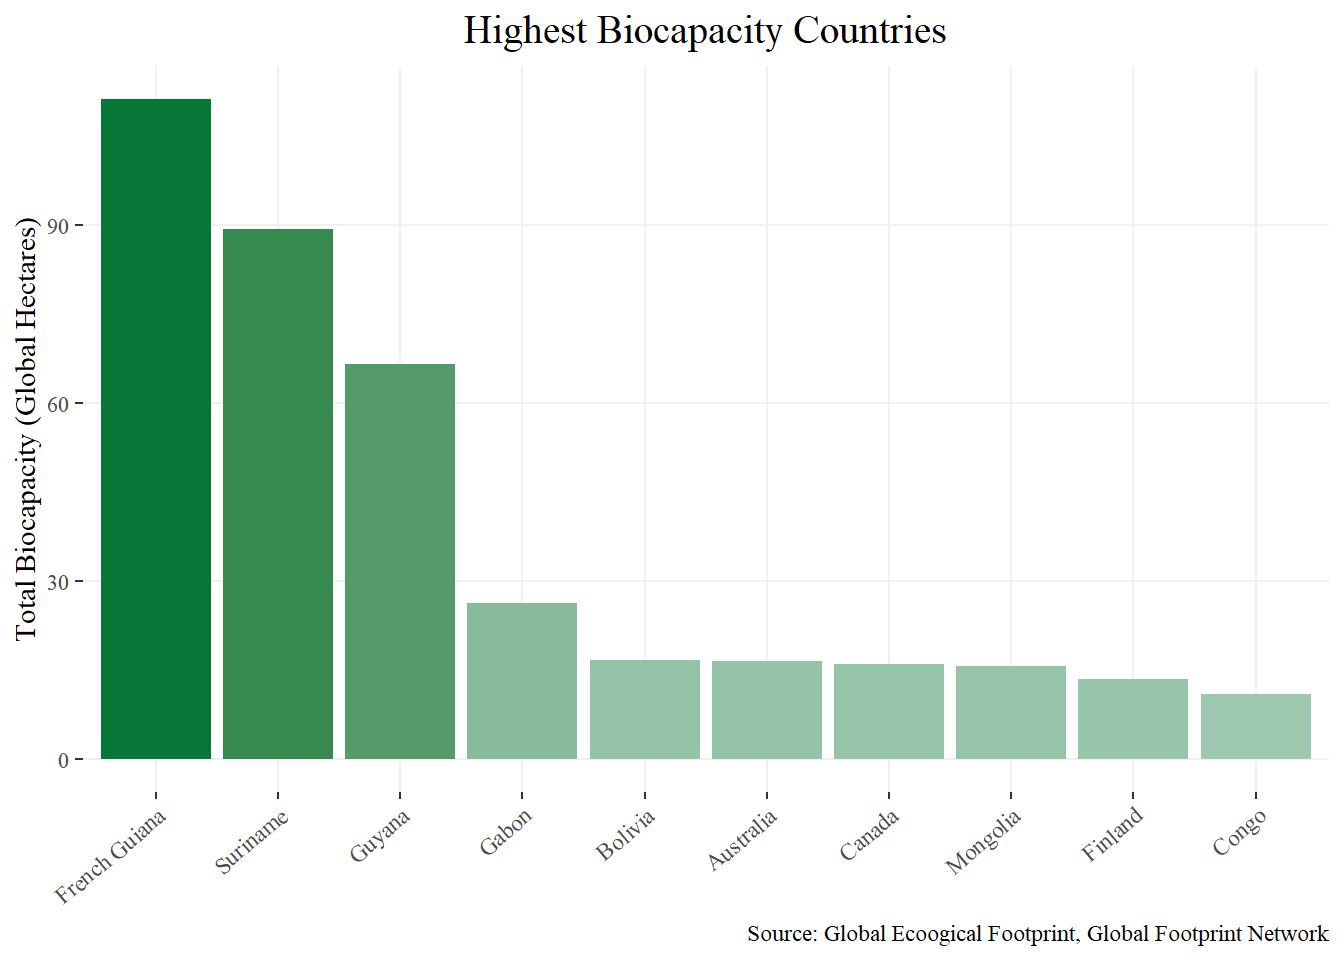
\includegraphics{footprint-paper_files/figure-latex/unnamed-chunk-4-1.pdf}

\hypertarget{relationship-between-hdi-and-ecological-footprintbiocapacity}{%
\subsection{Relationship between HDI and Ecological
Footprint/Biocapacity}\label{relationship-between-hdi-and-ecological-footprintbiocapacity}}

In this section, we look at the various relationships that are connected
to the main research question of this paper. Do HDI and GDP
(socio-economic factors) have a relationship with Ecological Footprint
or Biocapacity? While regression models will help with the inference for
particular countries, the dataset limits us here to do a cross-sectional
visualization. To add in more elements to the visualization, regionwise
categories and the population size (in millions) was added to the
scatter plot, giving us more dimensions to look at the data with.

This relationship is looked at by various scholars and researchers,
where the complicated issue of ecological footprint versus human
development is at the forefront. Kassouri and Altıntaş (2020) talk about
the presence of a strong trade-off between the ecological footprint and
human well-being captured by human development index. This is further
corroborated by Ahmad et al. (2020), who concluded that economic growth
and unrestricted usage of resources does lead to a growing ecological
footprint. This brings back to the question regarding the Sustainable
Development Goals, where countries vowed to progress with sustainability
in mind. Is this really the case? Developed nations spearheaded this
approach, and expected developing nations to follow their
recommendations.

From the resultant plots in this section, we can see a increasing
relationship when we look at HDI and ecological footprint. As HDI
increases on the X-axis, we see a resultant increase to the Y-axis which
shows the total Ecological Footprint of that corresponding nation. This
has interesting implications as the difference between economic growth
and development is fuzzy, and the HDI tries to look at a mixture of
variables which indicate both of them. However, does this also mean that
a growth in HDI would lead to better biocapacity in countries around the
world?

This is proven to be incorrect as seen from the second plot, which looks
at the relationship mentioned above. There is little evidence that all
regions increase in their biocapacity as was the case with the
ecological footprint. The implications for this is also interesting,
where we see that increasing HDI does not

\hypertarget{relationship-between-hdi-and-ecological-footprint}{%
\subsubsection{Relationship between HDI and Ecological
Footprint}\label{relationship-between-hdi-and-ecological-footprint}}

\begin{Shaded}
\begin{Highlighting}[]
\NormalTok{hdi1}\OtherTok{\textless{}{-}}\FunctionTok{ggplot}\NormalTok{(footprint) }\SpecialCharTok{+}
 \FunctionTok{aes}\NormalTok{(}\AttributeTok{x =}\NormalTok{ HDI, }\AttributeTok{y =}\NormalTok{ Total.Ecological.Footprint, }\AttributeTok{colour =}\NormalTok{ Region, }\AttributeTok{size =}\NormalTok{ Population.millions) }\SpecialCharTok{+}
 \FunctionTok{geom\_point}\NormalTok{(}\AttributeTok{shape =} \StringTok{"circle"}\NormalTok{) }\SpecialCharTok{+}
 \FunctionTok{scale\_color\_brewer}\NormalTok{(}\AttributeTok{palette =} \StringTok{"Dark2"}\NormalTok{, }\AttributeTok{direction =} \DecValTok{1}\NormalTok{) }\SpecialCharTok{+}
 \FunctionTok{labs}\NormalTok{(}\AttributeTok{x =} \StringTok{"HDI"}\NormalTok{, }
 \AttributeTok{y =} \StringTok{"Total Ecological Footprint (Global Hectares)"}\NormalTok{, }\AttributeTok{title =} \StringTok{"Relationship between HDI and Ecological Footprint"}\NormalTok{, }
 \AttributeTok{size =} \StringTok{"Population (Millions)"}\NormalTok{) }\SpecialCharTok{+}
\NormalTok{ ggthemes}\SpecialCharTok{::}\FunctionTok{theme\_gdocs}\NormalTok{()}\SpecialCharTok{+} \FunctionTok{theme}\NormalTok{(}\AttributeTok{plot.caption =} \FunctionTok{element\_text}\NormalTok{(}\AttributeTok{family =} \StringTok{"serif"}\NormalTok{,}
    \AttributeTok{hjust =} \FloatTok{1.25}\NormalTok{), }\AttributeTok{axis.title =} \FunctionTok{element\_text}\NormalTok{(}\AttributeTok{family =} \StringTok{"serif"}\NormalTok{,}
    \AttributeTok{colour =} \StringTok{"black"}\NormalTok{), }\AttributeTok{axis.text =} \FunctionTok{element\_text}\NormalTok{(}\AttributeTok{family =} \StringTok{"serif"}\NormalTok{),}
    \AttributeTok{axis.text.x =} \FunctionTok{element\_text}\NormalTok{(}\AttributeTok{family =} \StringTok{"serif"}\NormalTok{),}
    \AttributeTok{axis.text.y =} \FunctionTok{element\_text}\NormalTok{(}\AttributeTok{family =} \StringTok{"serif"}\NormalTok{),}
    \AttributeTok{plot.title =} \FunctionTok{element\_text}\NormalTok{(}\AttributeTok{family =} \StringTok{"serif"}\NormalTok{,}
        \AttributeTok{size =} \DecValTok{15}\NormalTok{, }\AttributeTok{colour =} \StringTok{"black"}\NormalTok{, }\AttributeTok{hjust =} \FloatTok{0.5}\NormalTok{),}
    \AttributeTok{legend.text =} \FunctionTok{element\_text}\NormalTok{(}\AttributeTok{family =} \StringTok{"serif"}\NormalTok{),}
    \AttributeTok{legend.title =} \FunctionTok{element\_text}\NormalTok{(}\AttributeTok{family =} \StringTok{"serif"}\NormalTok{)) }\SpecialCharTok{+}\FunctionTok{labs}\NormalTok{(}\AttributeTok{caption =} \StringTok{"Source: Global Footprint Network (GFN)"}\NormalTok{)}

\NormalTok{hdi1 }\SpecialCharTok{+} \FunctionTok{geom\_smooth}\NormalTok{(}\AttributeTok{se=}\ConstantTok{FALSE}\NormalTok{, }\AttributeTok{method=}\NormalTok{lm)}
\end{Highlighting}
\end{Shaded}

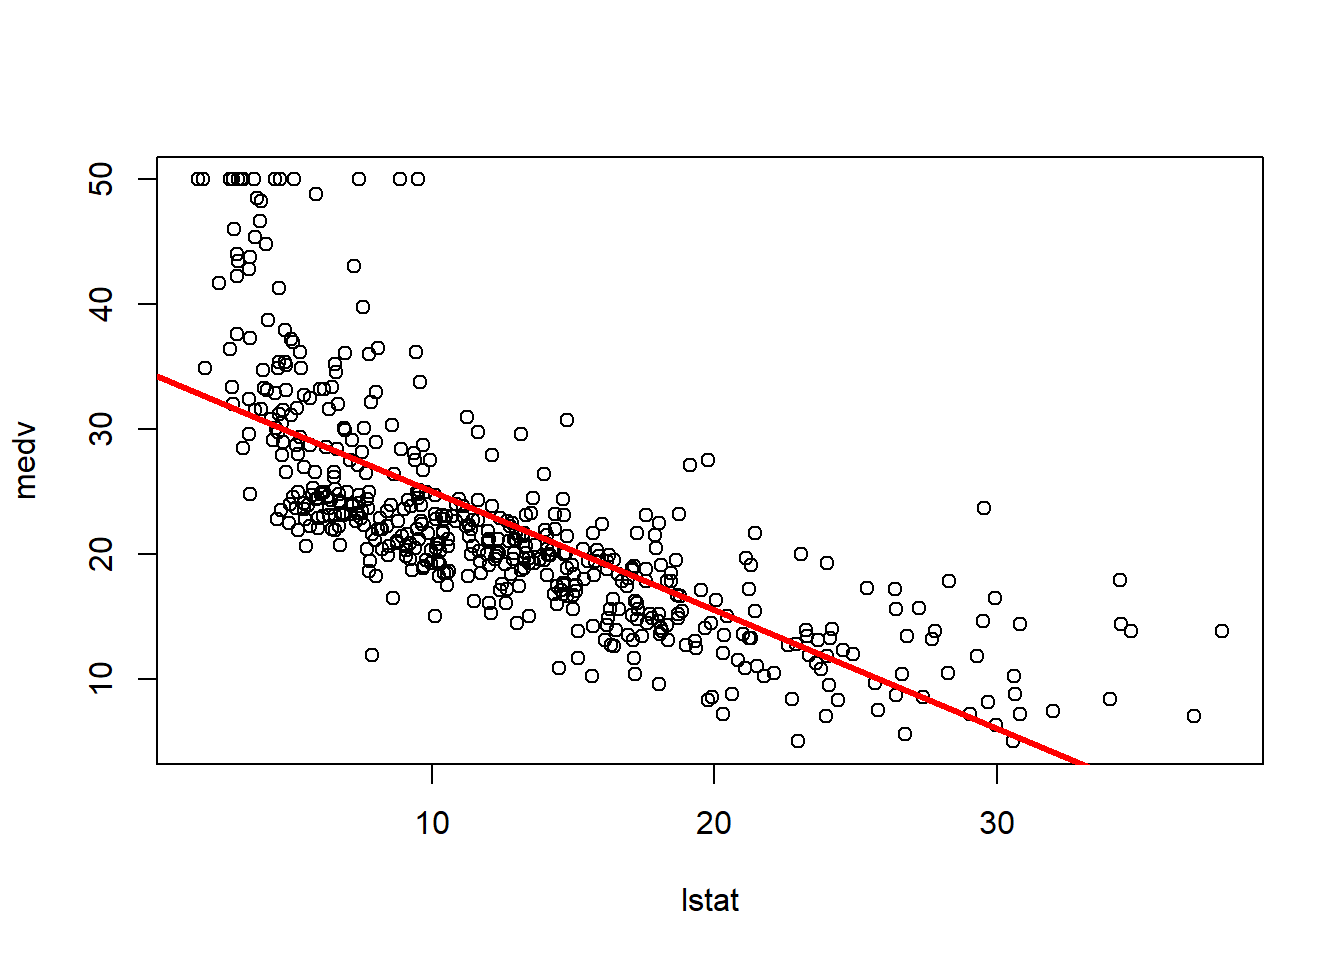
\includegraphics{footprint-paper_files/figure-latex/unnamed-chunk-5-1.pdf}

\hypertarget{relationship-between-hdi-and-biocapacity}{%
\subsubsection{Relationship between HDI and
Biocapacity}\label{relationship-between-hdi-and-biocapacity}}

\begin{Shaded}
\begin{Highlighting}[]
\NormalTok{hdi2}\OtherTok{\textless{}{-}}\FunctionTok{ggplot}\NormalTok{(footprint) }\SpecialCharTok{+}
  \FunctionTok{aes}\NormalTok{(}\AttributeTok{x =}\NormalTok{ HDI, }\AttributeTok{y =}\NormalTok{ Total.Biocapacity, }\AttributeTok{colour =}\NormalTok{ Region, }\AttributeTok{size =}\NormalTok{ Population.millions) }\SpecialCharTok{+}
  \FunctionTok{geom\_point}\NormalTok{(}\AttributeTok{shape =} \StringTok{"circle"}\NormalTok{) }\SpecialCharTok{+}
  \FunctionTok{scale\_color\_brewer}\NormalTok{(}\AttributeTok{palette =} \StringTok{"Dark2"}\NormalTok{, }\AttributeTok{direction =} \DecValTok{1}\NormalTok{) }\SpecialCharTok{+}
  \FunctionTok{labs}\NormalTok{(}\AttributeTok{x =} \StringTok{"HDI"}\NormalTok{, }
       \AttributeTok{y =} \StringTok{"Total Biocapacity (Global Hectares)"}\NormalTok{, }\AttributeTok{title =} \StringTok{"Relationship between HDI and Biocapacity"}\NormalTok{, }
       \AttributeTok{size =} \StringTok{"Population (Millions)"}\NormalTok{) }\SpecialCharTok{+}
\NormalTok{  ggthemes}\SpecialCharTok{::}\FunctionTok{theme\_gdocs}\NormalTok{()}\SpecialCharTok{+} \FunctionTok{theme}\NormalTok{(}\AttributeTok{plot.caption =} \FunctionTok{element\_text}\NormalTok{(}\AttributeTok{family =} \StringTok{"serif"}\NormalTok{,}
                                                             \AttributeTok{hjust =} \FloatTok{1.25}\NormalTok{), }\AttributeTok{axis.title =} \FunctionTok{element\_text}\NormalTok{(}\AttributeTok{family =} \StringTok{"serif"}\NormalTok{,}
                                                                                                      \AttributeTok{colour =} \StringTok{"black"}\NormalTok{), }\AttributeTok{axis.text =} \FunctionTok{element\_text}\NormalTok{(}\AttributeTok{family =} \StringTok{"serif"}\NormalTok{),}
                                 \AttributeTok{axis.text.x =} \FunctionTok{element\_text}\NormalTok{(}\AttributeTok{family =} \StringTok{"serif"}\NormalTok{),}
                                 \AttributeTok{axis.text.y =} \FunctionTok{element\_text}\NormalTok{(}\AttributeTok{family =} \StringTok{"serif"}\NormalTok{),}
                                 \AttributeTok{plot.title =} \FunctionTok{element\_text}\NormalTok{(}\AttributeTok{family =} \StringTok{"serif"}\NormalTok{,}
                                                           \AttributeTok{size =} \DecValTok{15}\NormalTok{, }\AttributeTok{colour =} \StringTok{"black"}\NormalTok{, }\AttributeTok{hjust =} \FloatTok{0.5}\NormalTok{),}
                                 \AttributeTok{legend.text =} \FunctionTok{element\_text}\NormalTok{(}\AttributeTok{family =} \StringTok{"serif"}\NormalTok{),}
                                 \AttributeTok{legend.title =} \FunctionTok{element\_text}\NormalTok{(}\AttributeTok{family =} \StringTok{"serif"}\NormalTok{)) }\SpecialCharTok{+}\FunctionTok{labs}\NormalTok{(}\AttributeTok{caption =} \StringTok{"Source: Global Footprint Network (GFN)"}\NormalTok{)}

\NormalTok{hdi2 }\SpecialCharTok{+} \FunctionTok{ylim}\NormalTok{(}\DecValTok{0}\NormalTok{,}\DecValTok{17}\NormalTok{) }\SpecialCharTok{+} \FunctionTok{geom\_smooth}\NormalTok{(}\AttributeTok{se=}\ConstantTok{FALSE}\NormalTok{, }\AttributeTok{method=}\NormalTok{lm)}
\end{Highlighting}
\end{Shaded}

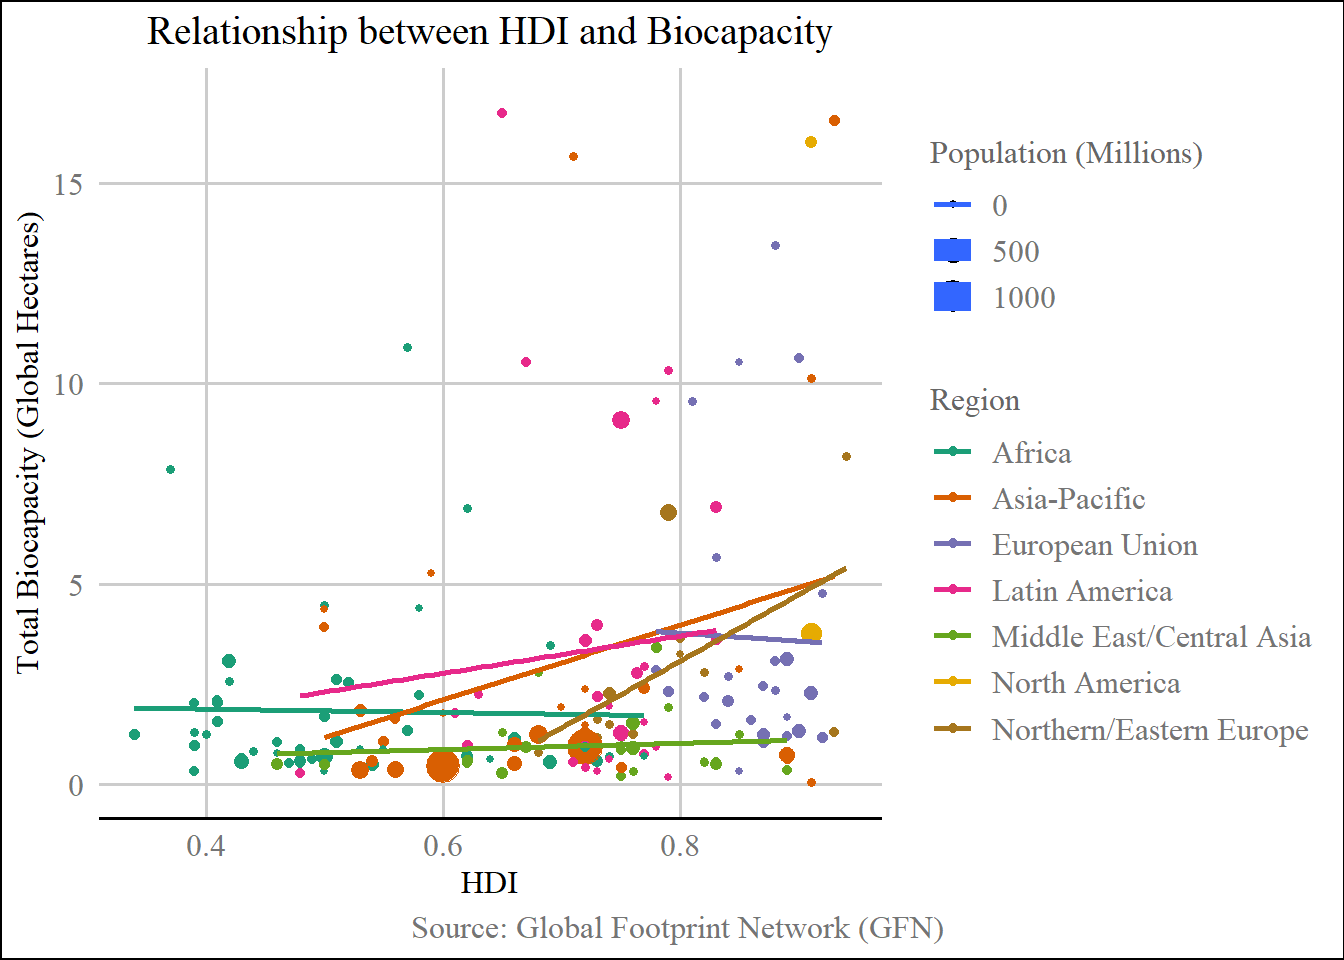
\includegraphics{footprint-paper_files/figure-latex/unnamed-chunk-6-1.pdf}

\hypertarget{relationship-between-gdp-per-capita-and-ecological-footprintbiocapacity}{%
\subsection{Relationship between GDP per Capita and Ecological
Footprint/Biocapacity}\label{relationship-between-gdp-per-capita-and-ecological-footprintbiocapacity}}

In this section, the second part of the research question will be looked
at. Do we see a connection between GDP per Capita, which is the
operationalization for economic growth and income growth, with the
Ecological Footprint or Biocapacity of nations? To further make the plot
interactive, the package \emph{plotly} is used, which gives us even more
access to look at the graph in greater detail. Here, a new variable -
the Ecological Deficit/Reserve, as was defined earlier in the paper.
Here, we once again return back to our original hypothesis - increase in
consumption leads to increased environmental impacts. This is the focus
for many researchers who try to look at specific industries that
negatively affect the environment, while at the same time not increasing
the biocapacity. Kubiszewski et al. (2013) look at historical data on
GDP and Ecological Footprint, where they surmise that efforts to
increase the GDP has led to there being a deficit when looking at
Ecological Footprint/Biocapacity. But as we move forward in the
technological age where innovation is the primary commodity being sold
between countries and sought after, will this remain the case?

Logic implies us to believe that efficiency increases will lead to a
reversal in the plots that are attached below. We see that there is a
positive correlation between GDP per Capita and Ecological Footprint,
where countries such as Luxembourg, Qatar, etc. have a deficit. However,
we can also see that Sweden and Australia have a Ecological reserve,
while having a high GDP per Capita. Highly technological countries which
have controlled for various other factors such as overpopulation,
resource management, etc. do stand a chance to reverse the trends that
we see here. In a paper by Szigeti, Toth, and Szabo (2017), the authors
have collated time series data and run tests that empirically prove that
there is a reversal happening. The authors mention efficiency gains due
to a technology variable which was not significant in earlier years of
the data.

\hypertarget{gdp-per-capita-ecological-footprint}{%
\subsubsection{GDP per Capita \& Ecological
Footprint}\label{gdp-per-capita-ecological-footprint}}

\begin{Shaded}
\begin{Highlighting}[]
\DocumentationTok{\#\# data cleaning}


\NormalTok{footprint1 }\OtherTok{\textless{}{-}}\NormalTok{ footprint }\SpecialCharTok{\%\textgreater{}\%}
  \FunctionTok{mutate}\NormalTok{(}\AttributeTok{Country =} \FunctionTok{as.character}\NormalTok{(Country), }\AttributeTok{GDP.per.Capita =} \FunctionTok{as.numeric}\NormalTok{(}\FunctionTok{gsub}\NormalTok{(}\StringTok{"[$,]"}\NormalTok{,}
                                                                           \StringTok{""}\NormalTok{, footprint}\SpecialCharTok{$}\NormalTok{GDP.per.Capita)), }\AttributeTok{HDI =} \FunctionTok{round}\NormalTok{(HDI,}
                                                                                                                       \DecValTok{2}\NormalTok{), }\AttributeTok{Countries.Required =} \FunctionTok{round}\NormalTok{(Countries.Required,}
                                                                                                                                                      \DecValTok{2}\NormalTok{), }\AttributeTok{Biocapacity.Deficit =} \FunctionTok{as.factor}\NormalTok{(}\FunctionTok{ifelse}\NormalTok{(Biocapacity.Deficit }\SpecialCharTok{\textgreater{}}
                                                                                                                                                                                                   \DecValTok{0}\NormalTok{, }\StringTok{"Reserve"}\NormalTok{, }\StringTok{"Deficit"}\NormalTok{))) }\SpecialCharTok{\%\textgreater{}\%}
  \FunctionTok{rename}\NormalTok{(}\AttributeTok{Status =}\NormalTok{ Biocapacity.Deficit) }\SpecialCharTok{\%\textgreater{}\%}
  \FunctionTok{select}\NormalTok{(}\SpecialCharTok{{-}}\FunctionTok{c}\NormalTok{(Data.Quality)) }\SpecialCharTok{\%\textgreater{}\%}
  \FunctionTok{drop\_na}\NormalTok{()}


\CommentTok{\# Scatterplot between GDP and Ecological Footprint}

\NormalTok{scat\_plot\_data }\OtherTok{\textless{}{-}}\NormalTok{ footprint1 }\SpecialCharTok{\%\textgreater{}\%}
  \FunctionTok{select}\NormalTok{(Country, Population.millions, GDP.per.Capita,}
\NormalTok{         HDI, Total.Ecological.Footprint, Status) }\SpecialCharTok{\%\textgreater{}\%}
  \FunctionTok{rename}\NormalTok{(}\AttributeTok{Population.in.millions =}\NormalTok{ Population.millions,}
         \AttributeTok{Human.Development.Index =}\NormalTok{ HDI, }\AttributeTok{Ecological.Footprint =}\NormalTok{ Total.Ecological.Footprint) }\SpecialCharTok{\%\textgreater{}\%}
  \FunctionTok{mutate}\NormalTok{(}\AttributeTok{text =} \FunctionTok{paste0}\NormalTok{(}\StringTok{"Country: "}\NormalTok{, Country, }\StringTok{"\textless{}br\textgreater{}"}\NormalTok{,}
                       \StringTok{"HDI: "}\NormalTok{, Human.Development.Index, }\StringTok{"\textless{}br\textgreater{}"}\NormalTok{, }\StringTok{"Ecological Footprint: "}\NormalTok{,}
\NormalTok{                       Ecological.Footprint, }\StringTok{"\textless{}br\textgreater{}"}\NormalTok{, }\StringTok{"GDP per Capita: "}\NormalTok{,}
                       \StringTok{"$"}\NormalTok{, GDP.per.Capita))}

\NormalTok{scat\_plot }\OtherTok{\textless{}{-}} \FunctionTok{ggplot}\NormalTok{(scat\_plot\_data, }\FunctionTok{aes}\NormalTok{(}\AttributeTok{x =}\NormalTok{ GDP.per.Capita,}
                                        \AttributeTok{y =}\NormalTok{ Ecological.Footprint, }\AttributeTok{text =}\NormalTok{ text)) }\SpecialCharTok{+} \FunctionTok{geom\_smooth}\NormalTok{(}\AttributeTok{col =} \StringTok{"\#61380B"}\NormalTok{,}
                                                                                              \AttributeTok{size =} \FloatTok{0.7}\NormalTok{) }\SpecialCharTok{+} \FunctionTok{geom\_point}\NormalTok{(}\FunctionTok{aes}\NormalTok{(}\AttributeTok{color =}\NormalTok{ Status, }\AttributeTok{size =}\NormalTok{ GDP.per.Capita)) }\SpecialCharTok{+}
  \FunctionTok{scale\_y\_continuous}\NormalTok{(}\AttributeTok{limits =} \FunctionTok{c}\NormalTok{(}\DecValTok{0}\NormalTok{, }\DecValTok{18}\NormalTok{)) }\SpecialCharTok{+} \FunctionTok{scale\_color\_manual}\NormalTok{(}\AttributeTok{values =} \FunctionTok{c}\NormalTok{(}\StringTok{"\#DF0101"}\NormalTok{,}
                                                                        \StringTok{"\#04B486"}\NormalTok{)) }\SpecialCharTok{+} \FunctionTok{labs}\NormalTok{(}\AttributeTok{title =} \StringTok{"GDP on Ecological Footprint"}\NormalTok{,}
                                                                                           \AttributeTok{y =} \StringTok{"Ecological Footprint"}\NormalTok{, }\AttributeTok{x =} \StringTok{"GDP Per Capita"}\NormalTok{) }\SpecialCharTok{+}
  \FunctionTok{theme}\NormalTok{(}\AttributeTok{plot.title =} \FunctionTok{element\_text}\NormalTok{(}\AttributeTok{face =} \StringTok{"bold"}\NormalTok{,}
                                  \AttributeTok{size =} \DecValTok{14}\NormalTok{, }\AttributeTok{hjust =} \DecValTok{0}\NormalTok{), }\AttributeTok{panel.background =} \FunctionTok{element\_rect}\NormalTok{(}\AttributeTok{fill =} \StringTok{"\#ffffff"}\NormalTok{),}
        \AttributeTok{panel.grid.major.x =} \FunctionTok{element\_line}\NormalTok{(}\AttributeTok{colour =} \StringTok{"grey"}\NormalTok{),}
        \AttributeTok{panel.grid.major.y =} \FunctionTok{element\_line}\NormalTok{(}\AttributeTok{colour =} \StringTok{"grey"}\NormalTok{),}
        \AttributeTok{axis.line.x =} \FunctionTok{element\_line}\NormalTok{(}\AttributeTok{color =} \StringTok{"grey"}\NormalTok{),}
        \AttributeTok{axis.line.y =} \FunctionTok{element\_line}\NormalTok{(}\AttributeTok{color =} \StringTok{"grey"}\NormalTok{),}
        \AttributeTok{axis.text =} \FunctionTok{element\_text}\NormalTok{(}\AttributeTok{size =} \DecValTok{10}\NormalTok{, }\AttributeTok{colour =} \StringTok{"black"}\NormalTok{),}
        \AttributeTok{legend.title =} \FunctionTok{element\_blank}\NormalTok{()) }\SpecialCharTok{+} \FunctionTok{theme}\NormalTok{(}\AttributeTok{axis.title =} \FunctionTok{element\_text}\NormalTok{(}\AttributeTok{family =} \StringTok{"serif"}\NormalTok{),}
    \AttributeTok{plot.title =} \FunctionTok{element\_text}\NormalTok{(}\AttributeTok{family =} \StringTok{"serif"}\NormalTok{,}
        \AttributeTok{size =} \DecValTok{15}\NormalTok{, }\AttributeTok{face =} \StringTok{"plain"}\NormalTok{, }\AttributeTok{hjust =} \FloatTok{0.5}\NormalTok{),}
    \AttributeTok{legend.text =} \FunctionTok{element\_text}\NormalTok{(}\AttributeTok{family =} \StringTok{"serif"}\NormalTok{),}
    \AttributeTok{legend.title =} \FunctionTok{element\_text}\NormalTok{(}\AttributeTok{family =} \StringTok{"serif"}\NormalTok{))}

\FunctionTok{ggplotly}\NormalTok{(scat\_plot, }\AttributeTok{tooltip =} \StringTok{"text"}\NormalTok{) }\SpecialCharTok{\%\textgreater{}\%}
  \FunctionTok{layout}\NormalTok{(}\AttributeTok{legend =} \FunctionTok{list}\NormalTok{(}\AttributeTok{orientation =} \StringTok{"v"}\NormalTok{, }\AttributeTok{y =} \DecValTok{1}\NormalTok{,}
                       \AttributeTok{x =} \DecValTok{0}\NormalTok{))}
\end{Highlighting}
\end{Shaded}

\hypertarget{gdp-per-capita-biocapacity}{%
\subsubsection{GDP per Capita \&
Biocapacity}\label{gdp-per-capita-biocapacity}}

\begin{Shaded}
\begin{Highlighting}[]
\NormalTok{scat\_plot\_data1 }\OtherTok{\textless{}{-}}\NormalTok{ footprint1 }\SpecialCharTok{\%\textgreater{}\%}
  \FunctionTok{select}\NormalTok{(Country, Population.millions, GDP.per.Capita,}
\NormalTok{         HDI, Total.Biocapacity, Status) }\SpecialCharTok{\%\textgreater{}\%}
  \FunctionTok{rename}\NormalTok{(}\AttributeTok{Population.in.millions =}\NormalTok{ Population.millions,}
         \AttributeTok{Human.Development.Index =}\NormalTok{ HDI, }\AttributeTok{Biocapacity =}\NormalTok{ Total.Biocapacity) }\SpecialCharTok{\%\textgreater{}\%}
  \FunctionTok{mutate}\NormalTok{(}\AttributeTok{text =} \FunctionTok{paste0}\NormalTok{(}\StringTok{"Country: "}\NormalTok{, Country, }\StringTok{"\textless{}br\textgreater{}"}\NormalTok{,}
                       \StringTok{"HDI: "}\NormalTok{, Human.Development.Index, }\StringTok{"\textless{}br\textgreater{}"}\NormalTok{, }\StringTok{"Biocapacity: "}\NormalTok{,}
\NormalTok{                       Biocapacity, }\StringTok{"\textless{}br\textgreater{}"}\NormalTok{, }\StringTok{"GDP per Capita: "}\NormalTok{,}
                       \StringTok{"$"}\NormalTok{, GDP.per.Capita))}

\NormalTok{scat\_plot1 }\OtherTok{\textless{}{-}} \FunctionTok{ggplot}\NormalTok{(scat\_plot\_data1, }\FunctionTok{aes}\NormalTok{(}\AttributeTok{x =}\NormalTok{ GDP.per.Capita,}
                                        \AttributeTok{y =}\NormalTok{ Biocapacity, }\AttributeTok{text =}\NormalTok{ text)) }\SpecialCharTok{+} \FunctionTok{geom\_smooth}\NormalTok{(}\AttributeTok{col =} \StringTok{"\#61380B"}\NormalTok{,}
                                                                                              \AttributeTok{size =} \FloatTok{0.7}\NormalTok{) }\SpecialCharTok{+} \FunctionTok{geom\_point}\NormalTok{(}\FunctionTok{aes}\NormalTok{(}\AttributeTok{color =}\NormalTok{ Status, }\AttributeTok{size =}\NormalTok{ GDP.per.Capita)) }\SpecialCharTok{+}
  \FunctionTok{scale\_y\_continuous}\NormalTok{(}\AttributeTok{limits =} \FunctionTok{c}\NormalTok{(}\DecValTok{0}\NormalTok{, }\DecValTok{18}\NormalTok{)) }\SpecialCharTok{+} \FunctionTok{scale\_color\_manual}\NormalTok{(}\AttributeTok{values =} \FunctionTok{c}\NormalTok{(}\StringTok{"\#DF0101"}\NormalTok{,}
                                                                        \StringTok{"\#04B486"}\NormalTok{)) }\SpecialCharTok{+} \FunctionTok{labs}\NormalTok{(}\AttributeTok{title =} \StringTok{"GDP on Biocapacity"}\NormalTok{,}
                                                                                           \AttributeTok{y =} \StringTok{"Biocapacity"}\NormalTok{, }\AttributeTok{x =} \StringTok{"GDP Per Capita"}\NormalTok{) }\SpecialCharTok{+}
  \FunctionTok{theme}\NormalTok{(}\AttributeTok{plot.title =} \FunctionTok{element\_text}\NormalTok{(}\AttributeTok{face =} \StringTok{"bold"}\NormalTok{,}
                                  \AttributeTok{size =} \DecValTok{14}\NormalTok{, }\AttributeTok{hjust =} \DecValTok{0}\NormalTok{), }\AttributeTok{panel.background =} \FunctionTok{element\_rect}\NormalTok{(}\AttributeTok{fill =} \StringTok{"\#ffffff"}\NormalTok{),}
        \AttributeTok{panel.grid.major.x =} \FunctionTok{element\_line}\NormalTok{(}\AttributeTok{colour =} \StringTok{"grey"}\NormalTok{),}
        \AttributeTok{panel.grid.major.y =} \FunctionTok{element\_line}\NormalTok{(}\AttributeTok{colour =} \StringTok{"grey"}\NormalTok{),}
        \AttributeTok{axis.line.x =} \FunctionTok{element\_line}\NormalTok{(}\AttributeTok{color =} \StringTok{"grey"}\NormalTok{),}
        \AttributeTok{axis.line.y =} \FunctionTok{element\_line}\NormalTok{(}\AttributeTok{color =} \StringTok{"grey"}\NormalTok{),}
        \AttributeTok{axis.text =} \FunctionTok{element\_text}\NormalTok{(}\AttributeTok{size =} \DecValTok{10}\NormalTok{, }\AttributeTok{colour =} \StringTok{"black"}\NormalTok{),}
        \AttributeTok{legend.title =} \FunctionTok{element\_blank}\NormalTok{()) }\SpecialCharTok{+} \FunctionTok{theme}\NormalTok{(}\AttributeTok{axis.title =} \FunctionTok{element\_text}\NormalTok{(}\AttributeTok{family =} \StringTok{"serif"}\NormalTok{),}
    \AttributeTok{plot.title =} \FunctionTok{element\_text}\NormalTok{(}\AttributeTok{family =} \StringTok{"serif"}\NormalTok{,}
        \AttributeTok{size =} \DecValTok{15}\NormalTok{, }\AttributeTok{face =} \StringTok{"plain"}\NormalTok{, }\AttributeTok{hjust =} \FloatTok{0.5}\NormalTok{),}
    \AttributeTok{legend.text =} \FunctionTok{element\_text}\NormalTok{(}\AttributeTok{family =} \StringTok{"serif"}\NormalTok{),}
    \AttributeTok{legend.title =} \FunctionTok{element\_text}\NormalTok{(}\AttributeTok{family =} \StringTok{"serif"}\NormalTok{))}

\FunctionTok{ggplotly}\NormalTok{(scat\_plot1, }\AttributeTok{tooltip =} \StringTok{"text"}\NormalTok{) }\SpecialCharTok{\%\textgreater{}\%}
  \FunctionTok{layout}\NormalTok{(}\AttributeTok{legend =} \FunctionTok{list}\NormalTok{(}\AttributeTok{orientation =} \StringTok{"v"}\NormalTok{, }\AttributeTok{y =} \DecValTok{1}\NormalTok{,}
                       \AttributeTok{x =} \DecValTok{0}\NormalTok{))}
\end{Highlighting}
\end{Shaded}

\hypertarget{references}{%
\section*{References}\label{references}}
\addcontentsline{toc}{section}{References}

\hypertarget{refs}{}
\begin{CSLReferences}{1}{0}
\leavevmode\hypertarget{ref-ahmad2020dynamic}{}%
Ahmad, Mahmood, Ping Jiang, Abdul Majeed, Muhammad Umar, Zeeshan Khan,
and Sulaman Muhammad. 2020. {``The Dynamic Impact of Natural Resources,
Technological Innovations and Economic Growth on Ecological Footprint:
An Advanced Panel Data Estimation.''} \emph{Resources Policy} 69:
101817.

\leavevmode\hypertarget{ref-galli2012assessing}{}%
Galli, Alessandro, Justin Kitzes, Valentina Niccolucci, Mathis
Wackernagel, Yoshihiko Wada, and Nadia Marchettini. 2012. {``Assessing
the Global Environmental Consequences of Economic Growth Through the
Ecological Footprint: A Focus on China and India.''} \emph{Ecological
Indicators} 17: 99--107.

\leavevmode\hypertarget{ref-unknown}{}%
Hild, Paula, Bianca Schmitt, Antoine Decoville, Morgane Mey, and Joëlle
Welfring. 2010. {``Ecological Footprint of Luxembourg -- Technical
Report.''} \url{https://doi.org/10.13140/RG.2.2.10249.95844}.

\leavevmode\hypertarget{ref-kassouri2020human}{}%
Kassouri, Yacouba, and Halil Altıntaş. 2020. {``Human Well-Being Versus
Ecological Footprint in MENA Countries: A Trade-Off?''} \emph{Journal of
Environmental Management} 263: 110405.

\leavevmode\hypertarget{ref-kubiszewski2013beyond}{}%
Kubiszewski, Ida, Robert Costanza, Carol Franco, Philip Lawn, John
Talberth, Tim Jackson, and Camille Aylmer. 2013. {``Beyond GDP:
Measuring and Achieving Global Genuine Progress.''} \emph{Ecological
Economics} 93: 57--68.

\leavevmode\hypertarget{ref-szigeti2017decoupling}{}%
Szigeti, Cecilia, Gergely Toth, and Daniel Robert Szabo. 2017.
{``Decoupling--Shifts in Ecological Footprint Intensity of Nations in
the Last Decade.''} \emph{Ecological Indicators} 72: 111--17.

\leavevmode\hypertarget{ref-toth2016historical}{}%
Toth, Gergely, and Cecı́lia Szigeti. 2016. {``The Historical Ecological
Footprint: From over-Population to over-Consumption.''} \emph{Ecological
Indicators} 60: 283--91.

\end{CSLReferences}

\end{document}
